\section{Preparation of muscle and system}\label{section_preparation}
\scp responses as a function of temperature. In order to precisely control the complicated system, electrical microprocessor was used. Therefore, in this section, the method for electrically operating \scp and investigating its characteristic is discussed. 

\subsection{Fabrication of \scp}
The \scp used in this paper was made by twisting silver-painted nylon thread (Conductive Sewing Thread Size 92, Shieldex), which were found to be best in terms of strain and force production \cite{haines}. First, as shown as Fig.\ref{silverSCP_1}, conductive thread was piled up four times to make its length be \SI{50}{\centi\meter}. Each side of thread was connected to washers. Then, wire was hung(Fig.\ref{silverSCP_2}) to one of the washer and motor to the other(Fig.\ref{silverSCP_3}). Motor was rotated until thread creates coil \cite{fab_coil}.(Fig.\ref{silverSCP_4}) After making same one again, two coils were overlapped to each other, making stable form.(Fig. \ref{silverSCP_5},\ref{silverSCP_6}) Lastly, by applying electric current, they were treated with heat.\footnote{\SI{2.5}{\ampere} of electric current was applied and stopped when smoke occurred. While repeating heating and cooling about ten times, the length at ambient temperature got longer and reaches constant length.} By this method, we made a \scp which is \SI{10}{\centi\meter} - \SI{11}{\centi\meter} in length and \SI{2.5}{\ohm} in electric resistance at ambient temperature with no external force.

\begin{figure}
	\centering
	\begin{minipage}{0.19\textwidth}
		\begin{subfigure}{\linewidth}
			\centering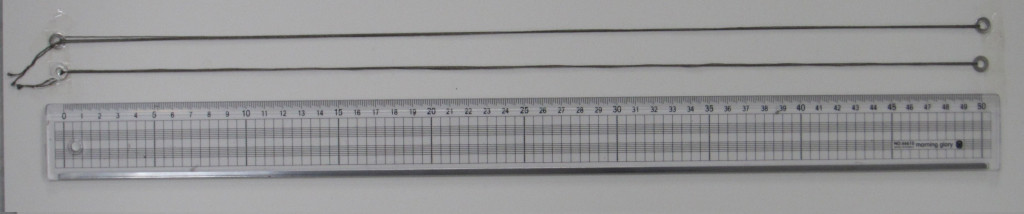
\includegraphics[width=\textwidth]{small_silverSCP_1.jpg}
			\caption{\label{silverSCP_1}}
		\end{subfigure}\\[2mm]
		\begin{subfigure}{\linewidth}
			\centering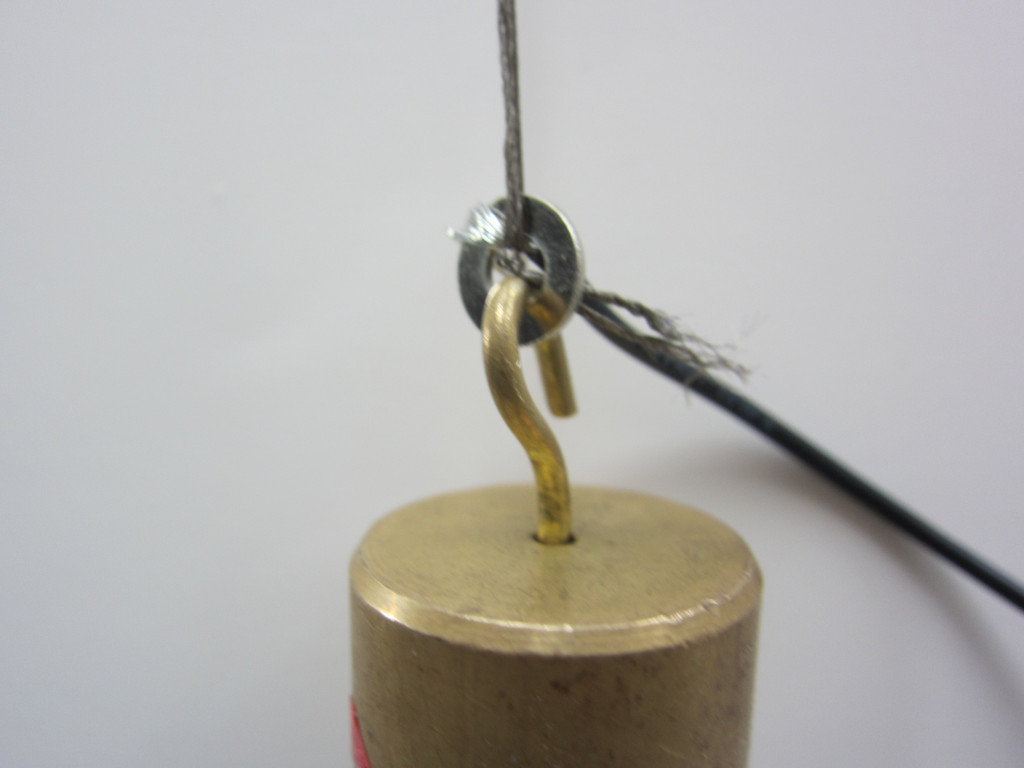
\includegraphics[width=\textwidth]{small_silverSCP_3.jpg}
			\caption{\label{silverSCP_2}}
		\end{subfigure}
	\end{minipage}%
	\begin{minipage}{.16\textwidth}
		\begin{subfigure}{\linewidth}
			\centering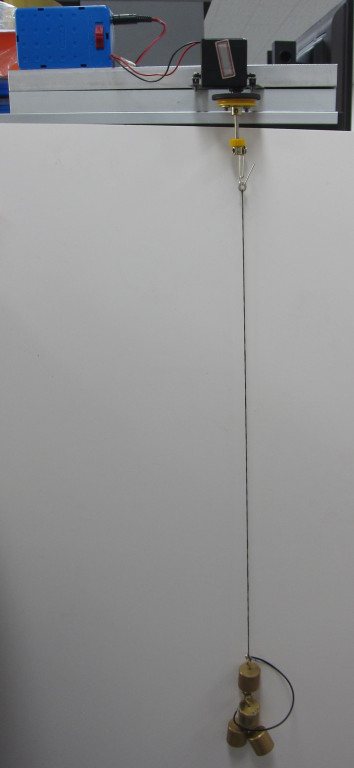
\includegraphics[height=3.7cm]{small_silverSCP_2.jpg}
			\caption{\label{silverSCP_3}}
		\end{subfigure}
	\end{minipage}%
	\begin{minipage}{.20\textwidth}
		\begin{subfigure}{\linewidth}
			\centering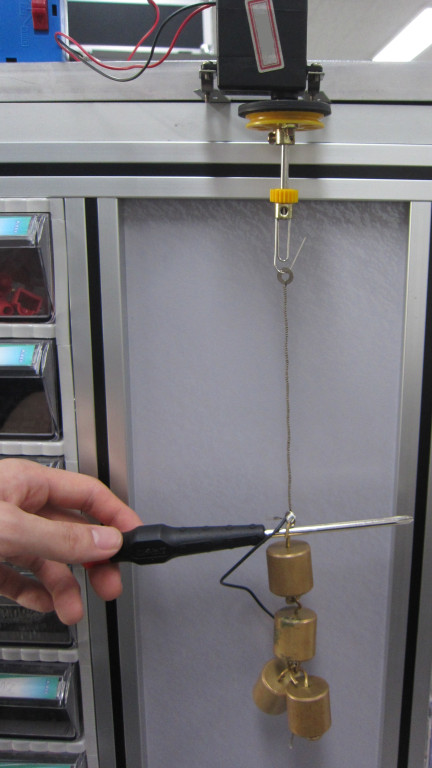
\includegraphics[height=3.7cm]{small_silverSCP_4.jpg}
			\caption{\label{silverSCP_4}}
		\end{subfigure}
	\end{minipage}%
	\begin{minipage}{.13\textwidth}
		\begin{subfigure}{\linewidth}
			\centering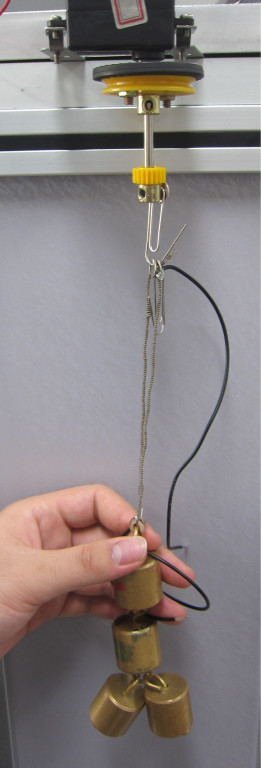
\includegraphics[height=3.7cm]{small_silverSCP_5.jpg}
			\caption{\label{silverSCP_5}}
		\end{subfigure}
	\end{minipage}%
	\begin{minipage}{.15\textwidth}
		\begin{subfigure}{\linewidth}
			\centering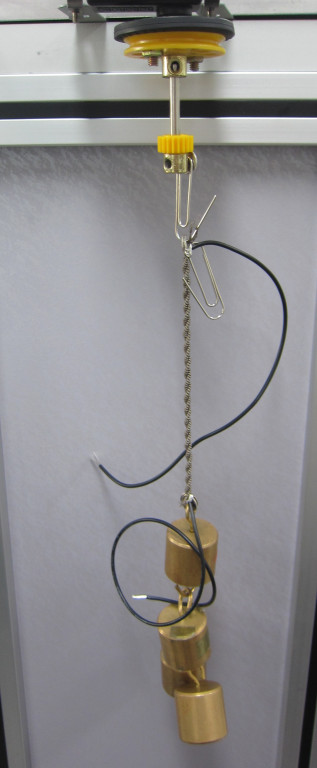
\includegraphics[height=3.7cm]{small_silverSCP_6.jpg}
			\caption{\label{silverSCP_6}}
		\end{subfigure}
	\end{minipage}%
	\begin{minipage}{.16\textwidth}
		\begin{subfigure}{\linewidth}
			\centering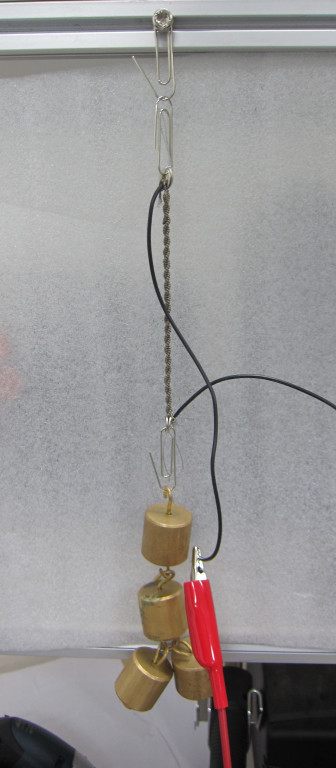
\includegraphics[height=3.7cm]{small_silverSCP_7.jpg}
			\caption{\label{silverSCP_anealing}}
		\end{subfigure}
	\end{minipage}%
	\caption[Process of making \scp with silver-painted nylon thread]{Process of making \scp with silver-painted nylon thread. \subref{silverSCP_1} 4-ply, \SI{50}{\centi\meter} thread bundle's each side was hung on washers. \subref{silverSCP_2}\subref{silverSCP_3} Up side was hung on motor, and down side was hung on \SI{400}{\gram} weight with wire inserted in between washer and thread. \subref{silverSCP_4} In order to twist thread until it creates coil, down side was fixed with a stick. \subref{silverSCP_5} By repeating process \subref{silverSCP_1} - \subref{silverSCP_4}, two super coiled polymer was made. Their up side were hung on one clip. Also, their down side were hung on \SI{400}{\gram} weight, which is same as \subref{silverSCP_3}. \subref{silverSCP_6} By these processes, \scp was made, which has wire on each side. \subref{silverSCP_anealing} Finally, they were annealed until length at ambient temperature doesn't get longer.}
	\label{silverSCP_makingof}
\end{figure}

\subsection{Electrical control of \scp}\label{section_electrical_control}
As discussed in previous section, \scp was made with conductive thread in order to electrically control heat speed. Electrical resistance of \scp was $R=\SI{2.5}{\ohm}$, so the power $P$ was supplied by applying voltage $V=\sqrt{PR}$. The voltage was controlled by MOSFET and PWM generation of Arduino Uno.

In order to implement faster cooling speed of \scp, compressed air tank and solenoid valve was used. Air tank forces air(temperature : equals to  $T_{ambient}$) to flow around \scp, so we can significantly increase the thermal conductivity $\lambda$ of muscle. Meanwhile, the amount of air flow can't be analog controlled. Therefore, by stopping and resuming flow of air with an appropriate period and ratio, we can control the thermal conductivity $\lambda$ of muscle. This will be discussed at section \ref{section_dynamic} on a closer view.

\subsection{Physical Measurements of \scp}
Physical properties of \scp, such as temperature, length, and tension, was measured with various sensors.
\footnote{For detail information of following sensors, see Table \ref{used_materials}.}
SMD type temperature sensor was used to measure the temperature of \scp without effecting the specific heat of \scp.

Also, slide potentiometer was used to measure the linear displacement of \scp. But, since it had significant amount of friction, it was only used for experiments about \scp's characteristics. On the other hand, rotary sensor, which had low frictional torque, was used to make an \anta. 

To measure the tension of \scp, load cell and amplifier was used.
Load cell played a role of connecting \scp and skeleton of \anta.
% As seen as Fig.\ref{anta_loadcell}, load cell played a role of connecting \scp and skeleton of \anta.

\subsection{An \ANTA}
\scp can be easily heated by applying electric current. However, cooling demands more sophisticated procedure. Also, muscles can only produce strong force while contracting. This means that \scp can't be directly applied to robots which have to produce force on various position. Therefore, we designed an \antanospace, so that the system is energy-optimal for various tasks \cite{antagonism}.

\begin{figure}[t]
	%add desired spacing between images, e. g. ~, \quad, \qquad, \hfill etc. 
	%(or a blank line to force the subfigure onto a new line)
	\centering
	\begin{subfigure}[t]{0.5\textwidth}
		\centering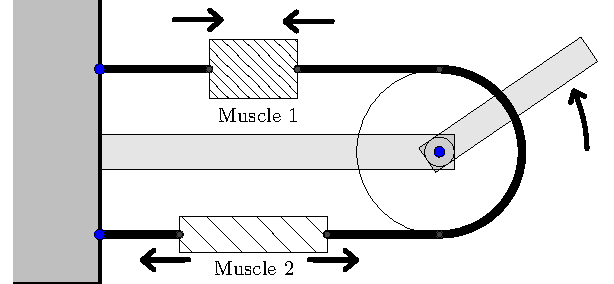
\includegraphics[width=\textwidth]{AntaSchematic_v3.pdf}
		\caption{\label{anta_sch}}
	\end{subfigure}
	~			
	\begin{subfigure}[t]{0.3\textwidth}
		\centering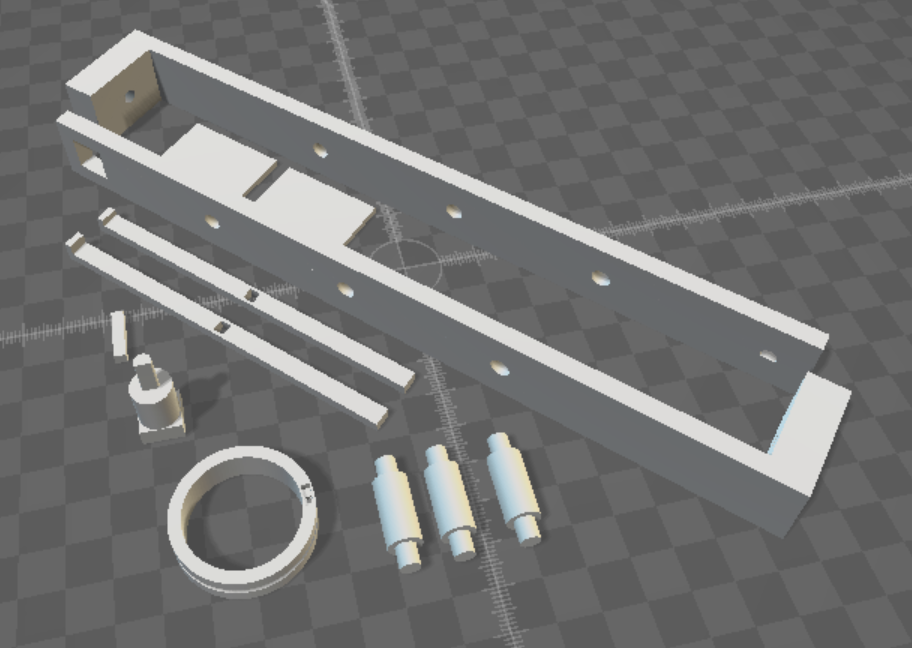
\includegraphics[width=\textwidth]{Anta_3d_assemblies_v2.png}
		\caption{\label{3d_assemblies}}
	\end{subfigure}
	
	\begin{subfigure}[t]{0.81\textwidth}
		\centering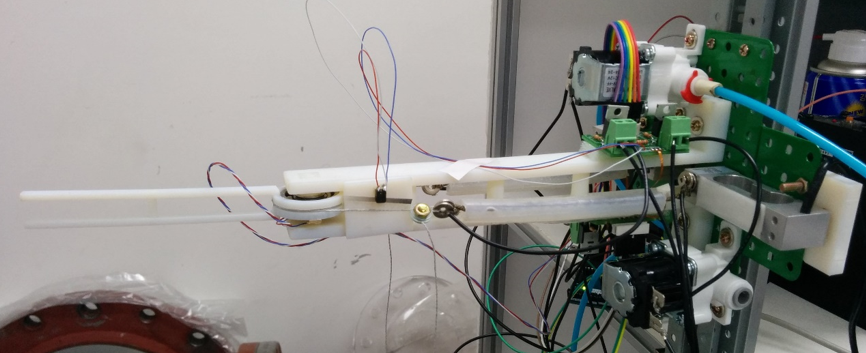
\includegraphics[width=\textwidth]{Anta_overall_v2.png}
		\caption{\label{anta_overall}}
	\end{subfigure}
	
	\caption[An \anta]{\subref{anta_sch} By contracting two \scpnospace s complementarily, we can get same effect of cooling one muscle by heating another. \subref{3d_assemblies} The skeleton of \anta was designed with software(3D Builder, Microsoft) and 3d-printed. \subref{anta_overall} An overall image of \anta.}
	\label{anta_design}
\end{figure}
